% AER-Article.tex for AEA last revised 22 June 2011
\documentclass[AER,draftmode]{AEA}

\usepackage{graphicx}
\usepackage{apacite}
\usepackage[colorinlistoftodos]{todonotes}

\usepackage{setspace}


% The mathtime package uses a Times font instead of Computer Modern.
% Uncomment the line below if you wish to use the mathtime package:
%\usepackage[cmbold]{mathtime}
% Note that miktex, by default, configures the mathtime package to use commercial fonts
% which you may not have. If you would like to use mathtime but you are seeing error
% messages about missing fonts (mtex.pfb, mtsy.pfb, or rmtmi.pfb) then please see
% the technical support document at http://www.aeaweb.org/templates/technical_support.pdf
% for instructions on fixing this problem.

% Note: you may use either harvard or natbib (but not both) to provide a wider
% variety of citation commands than latex supports natively. See below.

% Uncomment the next line to use the natbib package with bibtex 
%\usepackage{natbib}

% Uncomment the next line to use the harvard package with bibtex
%\usepackage[abbr]{harvard}

% This command determines the leading (vertical space between lines) in draft mode
% with 1.5 corresponding to "double" spacing.
\draftSpacing{1.5}
\setlength{\marginparwidth}{4cm}

\begin{document}

\title{Does Coverage of Sexual Assault Cases Ease the Reporting Decision? Evidence from FBI Data}
\shortTitle{Sexual Assault Reporting}
\author{Harry Elworthy\thanks{Duke University, harryelworthy@gmail.com.}}
\date{\today}
\pubMonth{}
\pubYear{}
\pubVolume{}
\pubIssue{}
\JEL{}
\Keywords{}

\begin{abstract}
Your abstract here.

Files available at \url{github.com/harryelworthy/Thesis}
\end{abstract}


\maketitle

%American Economic Review Pointers:

%\begin{itemize}
%\item Do not use an "Introduction" heading. Begin your introductory material
%before the first section heading.

%\item Avoid style markup (except sparingly for emphasis).

%\item Avoid using explicit vertical or horizontal space.

%\item Captions are short and go below figures but above tables.

%\item The tablenotes or figurenotes environments may be used below tables
%or figures, respectively, as demonstrated below.

%\item If you have difficulties with the mathtime package, adjust the package
%options appropriately for your platform. If you can't get it to work, just
%remove the package or see our technical support document online (please
%refer to the author instructions).

%\item If you are using an appendix, it goes last, after the bibliography.
%Use regular section headings to make the appendix headings.

%\item If you are not using an appendix, you may delete the appendix command
%and sample appendix section heading.

%\item Either the natbib package or the harvard package may be used with bibtex.
%To include one of these packages, uncomment the appropriate usepackage command
%above. Note: you can't use both packages at once or compile-time errors will result.

%\end{itemize}

\clearpage
An estimated 18.3\% of women and 1.4\% of men in the United States are sexually assaulted at some point in their lives, with more than a third of these assaults occurring before the victim turns 18  \cite{black_national_2011}. About 20\% to 25\% of women nationally are sexually assaulted at some point during their college careers \cite{fisher_sexual_2000}. At Duke, this figure is estimated at closer to 40\%, as well as 10\% of men \cite{fox_university_2017}. Despite this, very few assaults are reported to police. According to \citeA{fisher_sexual_2000}, "fewer than 5\% of attempted or completed sexual assault against college age women are reported to law enforcement. 66\% of victims tell friends but not family or school officials." \citeA{resnick_predictors_2000} finds that 1/5 of women that experience sexual assault report it to police, while \citeA{greenfield_sex_1997} estimates this number at 1/3 of women. Because these studies use self-reported survey data, there are still almost certainly non-reporting women and thus these estimates are likely upper bounds. Victims do not report to police for a number of reasons, discussed more in-depth below, including self-blame, guilt, fear of the perpetrator or fear of not being believed \cite{du_mont_role_2003}.

There are many reasons to seek to increase the proportion of sexual assaults that are reported. Some victims of of sexual assault do not want to report their crime to police because they do not wish their perpetrator to face justice, often because they are friends or are otherwise close. However, many victims would prefer to report their crime to the police, and balance this desire against the costs they see in reporting, costs summarized above and discussed in more depth below\todo{Need a source here}. There also obviously cannot be a criminal investigation if the crime is not reported to the police, and so women may wish to report in order to see justice for their assaulter. Victims of rape that report the crime to the police are also 9 times more likely to receive medical care than those that do not \cite{resnick_predictors_2000} as well as more likely to receive psychological care \cite{sable_barriers_2006} meaning that it is often in the interest of the victim's health for them to report the crime to police. Equally, there is a benefit to society of reporting. \citeA{bachman_factors_1998} notes that "an unreported incident of rape eliminates the possibility that an offender will be arrested or convicted. This may, in turn, reduce the perceived likelihood that rape and sexual assault, in general, will be punished." This reduction in perceived likelihood of punishment has significant consequences. A number of studies have found that the propensity of men to commit sexual assault is significantly decreased by the threat of formal sanctions such as arrest \cite{bachman_rationality_1992, antunes_impact_nodate}. Additionally, \citeA{abel_self-reported_1987} finds that non-incarcerated rapists have high recidivism rates, suggesting that unreported assaults pose a serious threat to others. Finally, increased reporting can be a sign that the barriers to reporting that victims feel, barriers often steeped in misogyny, are declining in severity. This is surely a thing to strive for.

Previous research has focused on many factors affecting the reporting decision, including relations of the victim to the perpetrator, whether the act was violent, whether alcohol was involved, and much more. This research is discussed more thoroughly in the next section. One factor not previously investigated, however, is the response of reporting behaviour to prominent coverage of sexual assault allegations and cases. The \#metoo movement that the Harvey Weinstein allegations started focused on women coming forward with their sexual assault stories because they saw others come forward with theirs - thus the 'me too.' This idea highlights an important question: are victims of sexual assault encouraged to report to police or other authorities by coverage of other victims reporting?

In this paper, I explore these questions using incident-level FBI data of crime reports from 2008 to 2016, along with search-volume data from Google Trends. I supplement this  with instrumental-variable analysis using a novel dataset of high-profile sexual assault allegations. 

\section{Background}

Since Becker outlined his economic model of crime, illicit activities have continued to have a place in the economic literature. Sexual assault has received a share of this attention, although perhaps less so than other crimes. One reason for this deficit is the difficulty of gathering accurate data on sexual assault. Crime is under-reported in general, sexual assault especially \cite{fisher_sexual_2000}. This under-reporting makes the study of sexual assault inherently difficult, because no study will ever be able to accurately gauge how many assaults actually occurred over a given time period. Studies that use surveys to estimate this under-reporting are always subject to under-reporting of their own, as even simply answering a survey question about sexual assault is difficult for many victims.\todo{Need source} When observing an increase in reports, the inability to observe assault numbers also creates issues of inference. Are reports increasing because people feel more safe reporting their assaults, or because assaults themselves are increasing? Different papers approach these issues in different ways when dealing with sexual assault.

Recently, several papers in economics have focused on sexual assault and harassment. \citeA{lindo_college_2018} looks at the effect of partying culture on reports of sexual assault using the plausible exogeneity of Division 1 football games. The authors find a 28\% increase in rape reports associated with game days.\footnote{This paper also uses the FBI incident-level data, and I use their code in my analysis.} \cite{bi}
\begin{itemize}
    \item Discuss the Girja paper, prostitution and assault very shortly.
\end{itemize}
\citeA{allen_reporting_2007} investigates the factors that influence an individual's decision to report a rape to law enforcement using survey data from The National Sample of Rape Victims, completed in 1985 and released in 2000, and finds that victims will be more likely to report sexual assault given more 'social support and ancillary evidence associated with the crime.' \todo{More on this paper needed}


More attention is paid to the reporting decision by other fields, especially law. 
\begin{itemize}
    \item Summarize a number of papers here, Bachmann etc. Get 3 or 4 really concrete results
\end{itemize}

These studies have their limitations. 
\begin{itemize}
    \item Talk about self-reported surveys, low n, etc.
\end{itemize}

My paper aims to contribute to the literature by using actual reports to police as catalogued by the FBI rather than survey data. There are clear limitations to this approach as well, which I discuss in my conclusion section, but it does avoid many of the problems discussed above. \begin{itemize}
    \item Beef this up, address above limitations
\end{itemize}{}

This question of the effect that news coverage has is important. 
\begin{itemize}
    \item Add more about why this is important. Mostly: if the effect was negative, it would be pressing to reduce this coverage, as with suicide
\end{itemize}

Previous economic research has used search volume in similar ways.
\begin{itemize}
    \item Needed! Have close to nothing here
\end{itemize}

I'd also like to include something like Figure~\ref{figure:police_yearly} below.

\begin{figure}

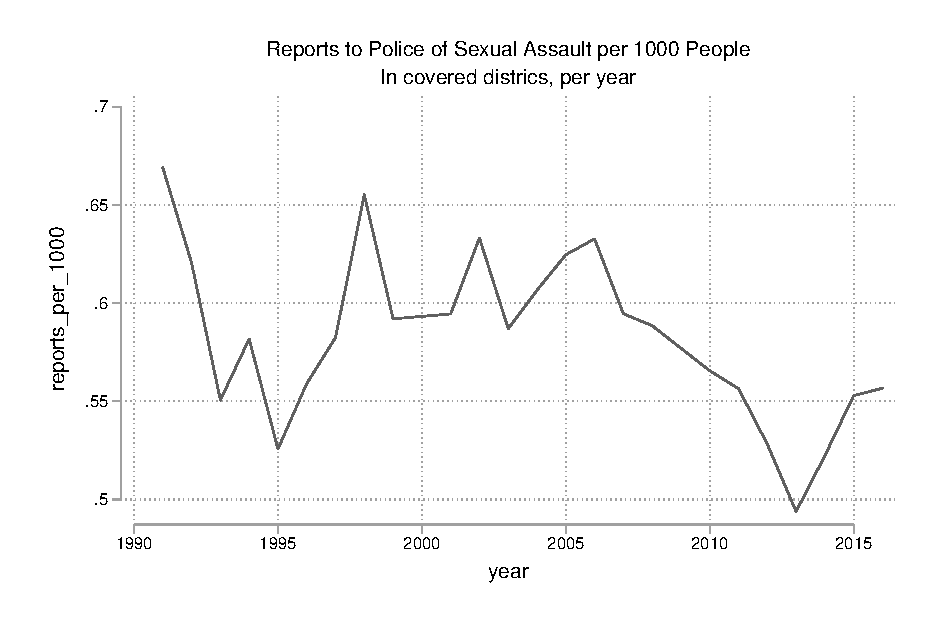
\includegraphics[width=\linewidth]{figures/police_yearly_reports.eps}

\caption{Reports to Police per Person, 1991 to 2015} \label{figure:police_yearly}
\end{figure}

\section{Data Summary}

I have two main data sources for this project: The National Incident-Based Reporting System (NIBRS) and relative search volumes from Google Trends. 

\begin{itemize}
    \item National Incident-Based Reporting System (NIBRS) Data
    \begin{itemize}
        \item Individual reports of crime to police stations. 1991 to 2016.
        \item About 40\% of population covered (some police stations don’t report) and this number has increased since 1991 as more stations have begun reporting.
        \item Timestamped, both report and incident datetime, lots of auxiliary information i.e. about the victim in question
        \item Because is by incident, can be collapsed to any specification: Nationally Daily, State-by-Week, etc. 
    \end{itemize}
    \item Google Trends data
    \begin{itemize}
        \item Daily and weekly trends for “sexual assault” 2008 to 2018 \footnote{Decided on "sexual assault" as "rape" tended to have a lot of unsavoury related searches, mostly pornography related, whereas searches for sexual assault tended to be related to cases of sexual assault. I test both for salience, and "rape" is not responsive to Title IX cases while "sexual assault" is. May try to add both back in.} \todo{Can probably change this to 2004 as not using News, need to rerun}
        \item National and statewide trends.
        \item Relative trends out of 100, scaled to 2008 numbers, so some numbers later on are higher.
        \item Merge daily with police data for most of my investigation. Thus have reports of sexual assault grouped by either report or incident date together with Google Trends, daily, from 2008 to 2016. 
    \end{itemize}
\end{itemize}

I'd like to have a small table of summary statistics here.

\section{Methodology}

In the first half of this section I'll discuss sexual assault, both the crime and the reporting of it, from an economic standpoint. This is outlined below. Second half, I outline the regression equations I'll be using.

\begin{itemize}
    \item Discussion of why someone might not report, fueled by \citeA{allen_reporting_2007} (where we see that a social safety net helps ease the reporting decision among other things) and \citeA{du_mont_role_2003} as well as any other papers I find about this
    \item Pull that discussion into a more formal discussion of the costs and uncertainty that one faces in reporting, and how coverage of sexual assault might affect that in one way or another: by lowering or raising expected cost of social stigma, by inspiring and perhaps increasing expected benefit, the idea that reporting can help reduce sexual assault. More here, need to come up with as exhaustive a list as I can, as this is important.
    \item Then spend some time discussing a similar thing but for potential perpetators - expected cost of assault. Obviously even more than the other one this is a behaviour that is tough to rationalize, but it's not wild to think (and one would seriously hope) that at the margin these people can be influenced one way or another
    \item Talk about the two in tandem, and again why hopefully reporting affects the second, and thus is important. If possible, this link would be great to try to estimate, but very difficult given the nature of the data. 
\end{itemize}

My initial regressions are time series regressions. They are at the daily level, and are of the form: 

$$ 
y_{t} = \beta_{0} + \sum_{b=-7}^{7} \delta_{b} x_{t+b} + \gamma_{t} + \varepsilon_{t}
$$

Where $y_{t}$ is the outcome variable in question; $x_{t+b}$ is the independent variable in question along with a set of leads and lags, and $\gamma{t}$ is a vector including day-of-week, week-of-year and year fixed-effects. These fixed effects should take care of most seasonality in the data. I include 7 leads and lags as a way to account for events happening in close proximity to each other without reducing degrees of freedom unnecessarily.

To accompany these time series results, I find events that are plausibly exogenous shocks to the volume of coverage of sexual assault-related topics, and use these shocks to instrument for the effect of an increase in such coverage on numbers of reports of sexual assault. These events are collected using Google's "Related Queries" function, that collects searches that are made in conjunction with the term in question over a specified time period. I look at times at which the Google Trend for 'sexual assault' is above 60\% of its 6-month maximum for the 9 years in question, which gives 563 days. For each day, I look for distinct related queries. For example, on November 19, 2014, 'Bill Cosby' is the top related query, as he is for the next several days. I count only the first occurrence of these terms as a distinct 'high profile event.' 

To use these events as instruments for the Google Trend, they must be correlated with the Google Trend and uncorrelated with the error term. To test the effect of these 'high profile events' on the Google Trend, I graph the response of the Trend before and after an event takes place, including fixed effects for year, week of year and day of week. This is shown in Figure~\ref{figure:events_trend}. As can be seen, these events have sizable effects on the Google Trend for 'sexual assault' that last for about 3 days. Thus they look to be good examples of random positive shocks to the google trend. To check whether reports seem to be impacted by these events occurring, I look at reports to police before and after these events in three day bins, including the same fixed effects as above. This is shown in Figure~\ref{figure:events_police_binned}. We see that reports do indeed increase around the date of an event, albeit with large standard errors. 

\begin{figure}
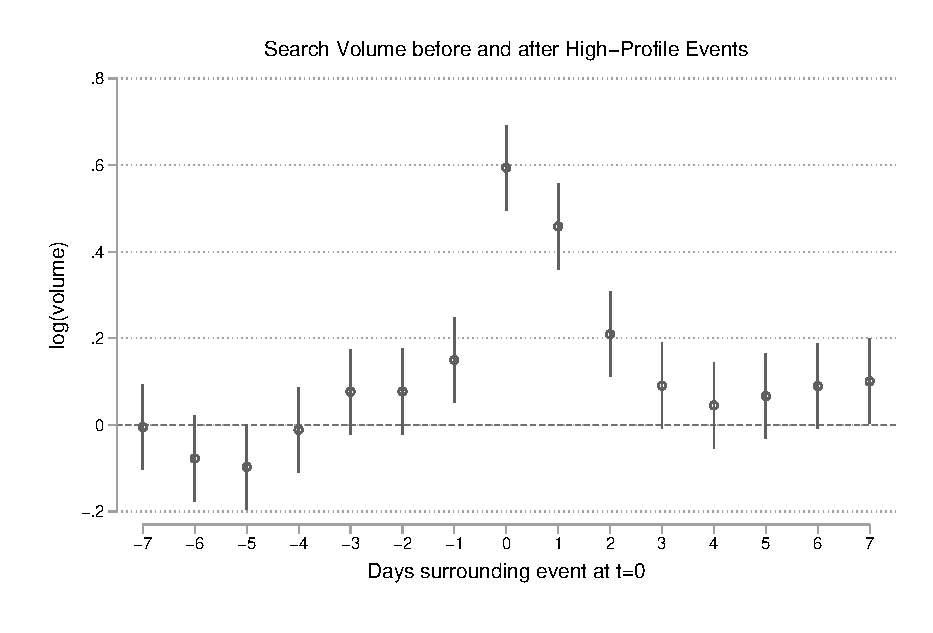
\includegraphics[width=\linewidth]{figures/events_trend.eps}
\caption{Google Trends before and after High Profile Events} \label{figure:events_trend}
\end{figure}

\begin{figure}
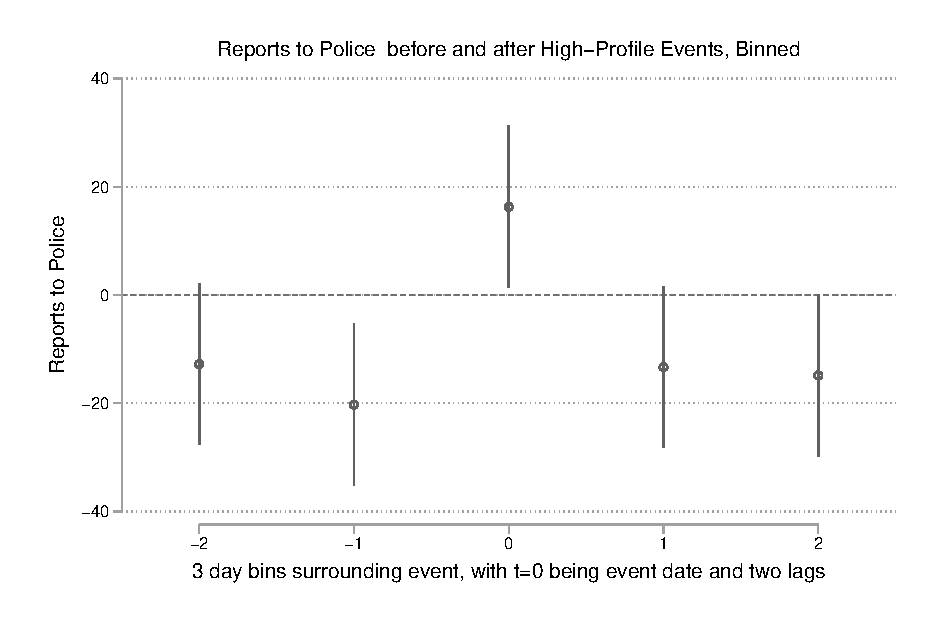
\includegraphics[width=\linewidth]{figures/events_police_binned.eps}
\caption{Reports to the FBI before and after High Profile Events, Binned} \label{figure:events_police_binned}
\end{figure}

\todo{Should have a discussion here about why this is plausibly exogenous, why it is not correlated with the error term, and why that is useful}

I use these events in a number of two stage least squares regressions. To take advantage of the 3 day window of significant effects on the Google Trend and reduce the standard errors of results, I bin results into the three day period including the event and two lag variables.

\todo{Outline here the first stage (different for each?) and the second stage, in equations}

My panel data regressions are of the form: \todo{Remove if not showing, or at least check over}

$$ 
y_{i,t} = \beta_{0} + \sum_{b=-7}^{7} \delta_{b} x_{i,t+b} + \alpha_{i} + \gamma_{t} + \varepsilon_{i,t}
$$

Where $y_{i,t}$ is the outcome variable in question; $x_{i,t+b}$ is the independent variable in question along with a set of leads and lags, $\alpha_{i}$ is a fixed effect at the level of the panel, usually by state or by school, and $\gamma{t}$ is a vector including year fixed-effects, as well as day-of-week and week-of-year fixed effects if the data is at the daily level.

My event study regressions are of the form: \todo{LIKELY DELETE}

$$ 
y_{t} = \beta_{0} + \sum_{b=-7}^{7} \delta_{b} x_{t+b} + \gamma_{t} + \varepsilon_{t}
$$

Where $y_{t}$ is the outcome variable in question; $x_{t+b}$ is a dummy for the event in question along with a set of leads and lags, and $\gamma{t}$ is a vector including day-of-week, week-of-year and year fixed-effects.

\section{Results}

I begin by running a time-series regression of reports of sexual assault to the FBI by report-date on national Google Trends for 'sexual assault'\todo{How best to note that it is in log form? once at the start? In every graph, in axes, in title?}. The results of this are shown in Figure~\ref{figure:police_trends_daily_logboth}. There is a clear, statistically significant effect on the first lag variable. I show this effect, as well as the same effect broken down by subgroups of age and race of the victim and whether the event was reported as involving alcohol, in the first column of Table~\ref{table:combinedtable}. To complement this time series analysis, I perform the same subgroup analysis with two different instrumental variable specifications as discussed in the methodology section, shown in columns 2 and 3 of Table~\ref{table:combinedtable}.

\begin{figure}
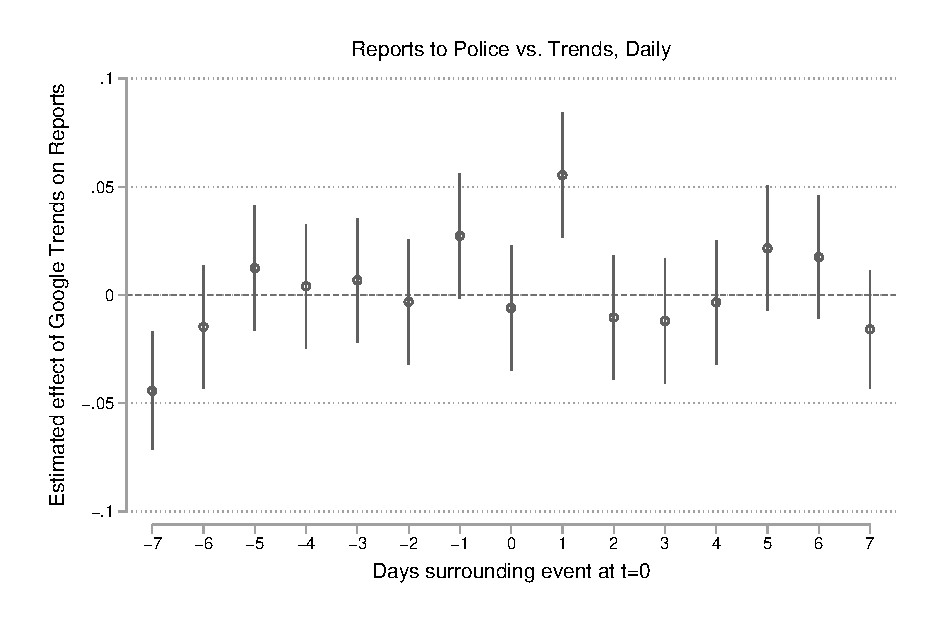
\includegraphics[width=\linewidth]{figures/police_trend_daily_logboth.eps}
\caption{Time-Series Regression of FBI Reports of Sexual Assault on Google Trends for 'sexual assault'} \label{figure:police_trends_daily_logboth}
\end{figure}

\begin{table}[]
\caption{Combined results of effect of increases in Google Trend on reports of sexual assault} \label{table:combinedtable}
{
\def\sym#1{\ifmmode^{#1}\else\(^{#1}\)\fi}
\begin{tabular}{l*{3}{c}}
\hline\hline
            &\multicolumn{1}{c}{(1)}&\multicolumn{1}{c}{(2)}&\multicolumn{1}{c}{(3)}\\
            &\multicolumn{1}{c}{log\_reports}&\multicolumn{1}{c}{log\_reports}&\multicolumn{1}{c}{log\_reports}\\
\hline
log\_trend   &      0.0568\sym{***}&       0.901\sym{*}  &      0.0521         \\
            &    (0.0146)         &     (0.434)         &    (0.0913)         \\
\hline
log\_trend\_10\_to\_19&      0.0611\sym{**} &       0.149         &     -0.0693         \\
            &    (0.0190)         &     (0.168)         &     (0.120)         \\
\hline
log\_trend\_20\_to\_29&      0.0315         &      0.0740         &      0.0104         \\
            &    (0.0196)         &     (0.169)         &     (0.129)         \\
\hline
log\_trend\_30\_to\_39&      0.0405         &      0.0109         &       0.226         \\
            &    (0.0280)         &     (0.240)         &     (0.176)         \\
\hline
log\_trend\_40\_to\_49&     -0.0324         &      -0.126         &      -0.471\sym{*}  \\
            &    (0.0369)         &     (0.315)         &     (0.223)         \\
\hline
log\_trend\_50\_to\_59&      0.0408         &       0.343         &       0.273         \\
            &    (0.0446)         &     (0.377)         &     (0.250)         \\
\hline
log\_trend\_60\_to\_69&      0.0320         &       0.179         &      -0.120         \\
            &    (0.0468)         &     (0.482)         &     (0.259)         \\
\hline
log\_trend\_white&      0.0578\sym{***}&       0.160         &       0.122         \\
            &    (0.0153)         &     (0.135)         &    (0.0970)         \\
\hline
log\_trend\_black&      0.0645\sym{**} &      0.0179         &     0.00573         \\
            &    (0.0233)         &     (0.201)         &     (0.140)         \\
\hline
log\_trend\_other&      0.0389         &      -0.122         &      -0.728\sym{**} \\
            &    (0.0408)         &     (0.353)         &     (0.274)         \\
\hline
log\_trend\_alc&     -0.0176         &     -0.0565         &      -0.195         \\
            &    (0.0530)         &     (0.260)         &     (0.271)         \\
\hline
log\_trend\_non\_alc&     -0.0176         &     -0.0565         &      -0.195         \\
            &    (0.0530)         &     (0.260)         &     (0.271)         \\
\hline
\(N\)       &        3288         &        3289         &        3289         \\
adj. \(R^{2}\)&       0.273         &           .         &       0.190         \\
\hline\hline
\multicolumn{4}{l}{\footnotesize Standard errors in parentheses}\\
\multicolumn{4}{l}{\footnotesize \sym{*} \(p<0.05\), \sym{**} \(p<0.01\), \sym{***} \(p<0.001\)}\\
\end{tabular}
}

\end{table}

All three specifications give positive coefficients for the overall effect, ranging in magnitude from 0.0568 to 0.219. To contextualize this, the mean daily number of reports per day from 2008 to 2016 was 110. \todo{Would median be more appropriate here?} According to the low estimate, a 1\% increase in the search volume for 'sexual assault' for a day leads to an increase of 0.062 reports, while the high estimate gives an increase of 0.24 reports. Given that the NIBRS data only covers 1/4 of the US, if we assume a homogenous effect across the country, these estimates become 0.25 and 0.96 reports respectively.

To give further context, the increases in search volume depicted in Figure~\ref{figure:events_trend} give an average increase in search volume of 42\% over the day of the event and the two days following. Given these increases, one of these events occurring will result in a spike of between 31 and 121 reports nationally, according to my low and high estimates respectively. For 'big allegations,' these estimates are 46 and 178 reports nationally. \todo{Explain how I picked big allegations}

This increase appears to be driven by white reporters under 20 and to a lesser extent under 30, reporting incidents that did not involve alcohol. There are, however, significant limitations with this sub-group analysis. \todo{Beef up paragraph, explain that most null results likely because of lower n, explain what we can maybe see, i.e. young, white, non-alc victims definitely affected, all likely more than proportionally. Middle age people do not look like they are affected as much.}

I next look at variation in effect by state, to try to determine whether states with relatively higher trends on a given day have higher numbers of reports. \todo{Bad sentence here} I consider this using both a normal panel regression and using the same instrument as in Model 2 above. \footnote{I could not use the Model 3 with the panel dataset as there were two many collinearity issues.} Results are shown in Table~\ref{table:state_daily}. I fail to find significant results using either model, indicating that coverage at a more local level may not have the effects that national coverage does.

\begin{table}[]
\caption{Effect of increases in state Google Trend on reports of sexual assault} \label{table:state_daily}
{
\def\sym#1{\ifmmode^{#1}\else\(^{#1}\)\fi}
\begin{tabular}{l*{1}{c}}
\hline\hline
            &\multicolumn{1}{c}{(OLS)}\\
            &\multicolumn{1}{c}{log\_reports}\\
\hline
log\_trend   &    -0.00422         \\
            &    (0.0289)         \\
\hline
\(N\)       &        6676         \\
adj. \(R^{2}\)&      -0.300         \\
\hline\hline
\multicolumn{2}{l}{\footnotesize Standard errors in parentheses}\\
\multicolumn{2}{l}{\footnotesize \sym{*} \(p<0.05\), \sym{**} \(p<0.01\), \sym{***} \(p<0.001\)}\\
\end{tabular}
}

\end{table}

To test the robustness of my instrumental variable analysis, I run my regressions with a number of different time fixed effects. Results are shown in Table~\ref{table:iv_robust}. The first three columns are using instrumental method 1, and the next three use method 2. Columns 1 and 4 are using year and week-of-year fixed effects; columns 2 and 5 use monthly fixed effects; and columns 3 and 6 use weekly fixed effects. The first three columns also use day of week fixed effects - I can't use these when I use method 2, as discussed in footnote above\todo{refer to this footnote!!}. All results are still positive, although some of them lose their significance. This means that we can be very confident in the sign of our result, but not especially confident of its magnitude.\todo{Finish this up}

\begin{table}[]
\caption{Instrumental Variable Fixed Effects Robustness Checks} \label{table:iv_robust}
{
\def\sym#1{\ifmmode^{#1}\else\(^{#1}\)\fi}
\begin{tabular}{l*{6}{c}}
\hline\hline
            &\multicolumn{1}{c}{(1)}&\multicolumn{1}{c}{(2)}&\multicolumn{1}{c}{(3)}&\multicolumn{1}{c}{(4)}&\multicolumn{1}{c}{(5)}&\multicolumn{1}{c}{(6)}\\
            &\multicolumn{1}{c}{log\_reports}&\multicolumn{1}{c}{log\_reports}&\multicolumn{1}{c}{log\_reports}&\multicolumn{1}{c}{log\_reports}&\multicolumn{1}{c}{log\_reports}&\multicolumn{1}{c}{log\_reports}\\
\hline
log\_trend   &      0.0885         &      0.0907         &       0.219\sym{**} &      0.0620         &      0.0519         &       0.140\sym{**} \\
            &    (0.0475)         &    (0.0582)         &    (0.0777)         &    (0.0350)         &    (0.0443)         &    (0.0510)         \\
[1em]
\_cons      &       4.586\sym{***}&       4.232\sym{***}&       3.715\sym{***}&       4.723\sym{***}&       4.430\sym{***}&       4.048\sym{***}\\
            &     (0.196)         &     (0.251)         &     (0.313)         &     (0.154)         &     (0.204)         &     (0.223)         \\
\hline
\(N\)       &        3288         &        3288         &        3288         &        3288         &        3288         &        3288         \\
adj. \(R^{2}\)&       0.262         &       0.191         &       0.170         &       0.241         &       0.173         &       0.165         \\
\hline\hline
\multicolumn{7}{l}{\footnotesize Standard errors in parentheses}\\
\multicolumn{7}{l}{\footnotesize \sym{*} \(p<0.05\), \sym{**} \(p<0.01\), \sym{***} \(p<0.001\)}\\
\end{tabular}
}

\end{table}

\clearpage
\section{Extra figures and results}

Below I look at incident dates of incidents reported within a month after a high profile event, compared to the same for a sample of placebo dates. Trying to work out how to interpret this, and add error bars. \todo{Probably refer to this in conclusion under next possible steps}

\begin{figure}
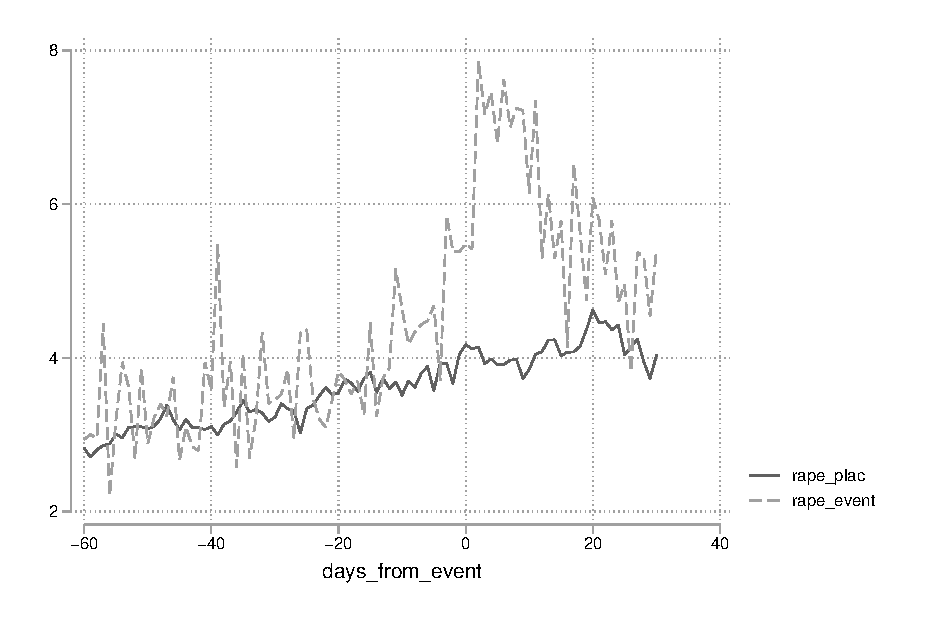
\includegraphics[width=\linewidth]{figures/idt_analysis_2.eps}
\end{figure}


Bring up school reporting again? Don't think so. If I did my narrative would go something like this:
\begin{itemize}
    \item Maybe we also see effects for much more local cases
    \item Potential evidencefor this: school reporting after title IX cases
    \item Show huge increase in reports at schools after title IX cases get opened there, explain that the cases are very salient as shown in \citeA{lindo_any_2018}
    \item However, looking closer this doesn't seem to hold up especially well
    \item Figure showing that effect is only on the first case, not subsequent ones
    \item Figures showing no increase in nearby schools or police stations (still need to rerun this, especially daily police) - maybe there is a small increase
\end{itemize}
If not, should have somewhere that school data was not feasible for x reasons (?)
\section{Discussion}

TBD

\clearpage
\section{To Discuss}

\begin{itemize}
    \item IDT analysis graph - hopefully. Otherwise methodology of it. Probably just qualitative. I'm found of using it as a way to discuss possible next steps.
    \item Talk about local/national T9 results with P Bayer. Bad news for my other results - other mechanisms? Although not the same type of event
    \item Talk about methodology on trend. Log? Original Trend?
    \item Best tables? Just one with overall effect, subgroups, columns are naive, instrument, log, log instrument? or something?
    \item Tables/Figures draft approx sequence
    \item Should make numbers national equivalent in tables? 
    \item Should I run with year interactions/something to check changing effect? Not that many years?
    \item IRF? Not sure I see what would be different than the graphs I have already
    \item Intro/Background/how to break up? How long intro?
    \item Summary statistics? What would be interesting?
\end{itemize}


\clearpage 
\section{Next Steps}

\begin{itemize}
    \item Run state fixed effects with weights by population (once decided) as well as state cases
    \item Finish idt\_analysis. Graph
    \item Do same for 50/100/200 random generated time segments depending on time the above takes, compare shapes
    \item Check results on population1 - use if not ridiculous
    \item Calculate average event effect, equivalent to the US. Note the assumption in homogeneous effect.
    \item Find any more 
    \item Write a paragraph on future work. More on perpetrator behavior. More on whether increased reports are true new reports or just earlier reports.
    \item Put in methodology/somewhere about how this may be people reporting more quickly, not new reports. Assume some are new at least.
    \item Include state panel data with date fixed effects somewhere - null
    \item Look for more high-profile cases for event study. Go back before 2008, re-go-over already done dates
\end{itemize}


% The appendix command is issued once, prior to all appendices, if any.
\clearpage
%References here (manual or bibTeX). If you are using bibTeX, add your bib file 
%name in place of BibFile in the bibliography command.
% Remove or comment out the next two lines if you are not using bibtex.

\bibliographystyle{apacite}
\bibliography{refs}

\clearpage
\appendix

\begin{table}[]
\caption{High Profile Events, collected using Google Related Trends on high-trend days}
{
\def\sym#1{\ifmmode^{#1}\else\(^{#1}\)\fi}
\begin{tabular}{llr}
\hline\hline
date       & name                                  & big\_event \\
\hline
21/07/2009 & Roethlisberger                        &            \\
09/03/2010 & Roethlisberger                  &            \\
30/09/2010 & MSU Athletes                          &            \\
22/11/2010 & Notre Dame Suicide  &            \\
16/02/2011 & Lara Logan   &            \\
29/11/2011 & Wellesley    &            \\
10/01/2012 & Joe Philbin son                       &            \\
01/04/2012 & SA Aware Month                        &            \\
15/05/2012 & Prosper TX athlete                    &            \\
18/10/2012 & Amherst Document                      &            \\
28/12/2012 & Case McCoy                            &            \\
19/01/2013 & Michael Crabtree                      &            \\
01/04/2013 & SA Aware Month                        &            \\
07/05/2013 & USAF                          &            \\
14/11/2013 & Jameis Winston                        & 1          \\
01/05/2014 & 55 colleges sexual assault            &            \\
10/09/2014 & Jerry Jones            &            \\
19/11/2014 & Bill Cosby                            & 1          \\
27/02/2015 & Scott Walker                          & 1          \\
25/03/2015 & Lara Logan           &            \\
27/03/2015 & Subway            &            \\
01/04/2015 & Bikram Choudhury                 &            \\
15/04/2015 & Panama City                      &            \\
21/05/2015 & Josh Duggar                           &            \\
21/09/2015 & College Climate paper released        &            \\
09/11/2015 & Biden Speech                            &            \\
23/11/2015 & Jameis Winston                 &            \\
02/12/2015 & James Deen                            &            \\
30/12/2015 & Bill Cosby                      & 1          \\
07/01/2016 & Cologne New Year Assaults             &            \\
12/01/2016 & David Bowie                           &            \\
13/02/2016 & Peyton Manning                        & 1          \\
29/02/2016 & Lady Gaga                             & 1          \\
01/04/2016 & SA Aware Month                        &            \\
13/04/2016 & Kobe Bryant                           &            \\
10/06/2016 & Stanford Student                      & 1          \\
08/10/2016 & Donald Trump                    & 1          \\
\hline\hline \\
\end{tabular}
}
\end{table}

\clearpage
\chapter{States included in FBI reporting}


\end{document}

